183. \begin{figure}[ht!]
\center{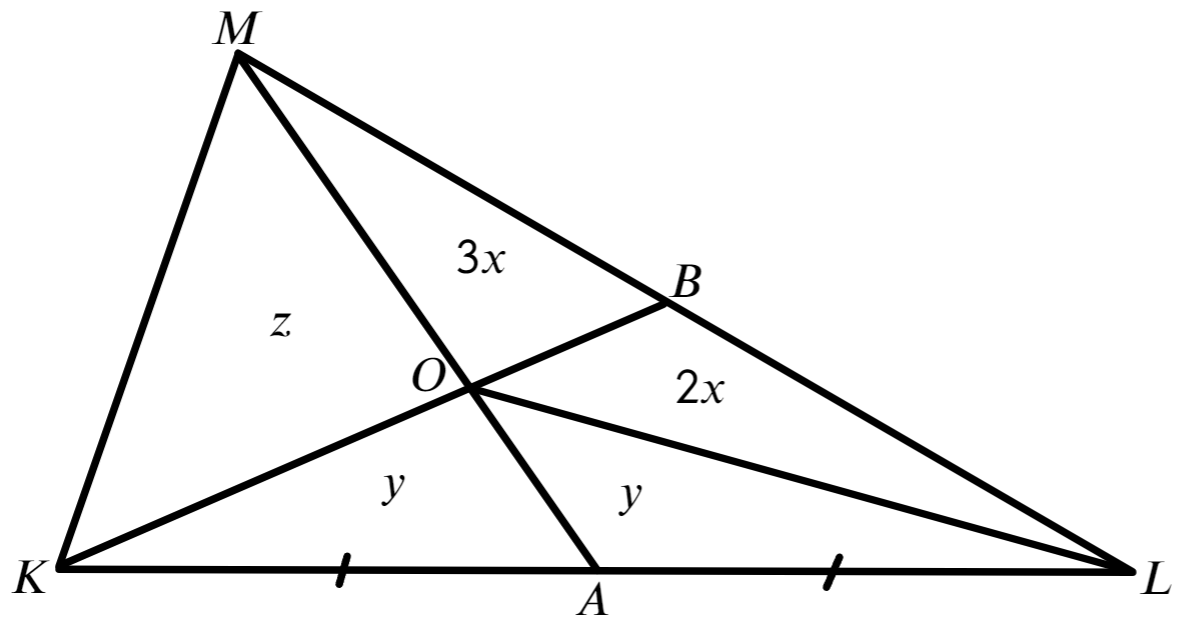
\includegraphics[scale=0.35]{g9-183.png}}
\end{figure}\\
Площади треугольников с общей высотой относятся так же, как стороны, на которые опущена эта высота, поэтому введём обозначения $S_{\Delta BOL}=2x,\ S_{\Delta BOM}=3x,\ S_{\Delta KOA}=S_{\Delta LOA}=y,\ S_{\Delta KMO}=z.$ Из треугольников $KMA$ и $LMA$ получим равенство $z+y=2x+3x+y,\ z=5x.$ Тогда $KO:OB=\cfrac{5x}{3x}=\cfrac{5}{3},$ откуда $KO:KB=5:8.$\\
